\documentclass[spanish,letterpaper,oneside]{article}

\def\documenttitle {¿Qué sabemos y cómo lo enseñamos?}
\def\documentsubtitle {Temas selectos de matemáticas I · Cohorte SD26}
\def\documentsubject {Actividad 1 (Sesión 8) · Retos de Área, Perímetro y Propuesta Canva}
\def\documentauthor {Mtro. Martín Jonathan de la Cruz Muñoz}
\def\coursename {Temas selectos de matemáticas I}
\def\coursecode {PFM02}

\def\universityname {Instituto de Investigación, Innovación y Estudios de Posgrado para la Educación del Estado de Nuevo León}
\def\universityfaculty {Maestría en Aprendizaje y Enseñanza de las Matemáticas}
\def\universitydepartment {Temas selectos de matemáticas I}
\def\universitydepartmentimage {img/iiiepe/marca-iiiepe.png}
\def\universitydepartmentimagecfg {height=1.75cm}
\def\universitylocation {Monterrey, Nuevo León}
\def\studentfullname {Mtro. Martín Jonathan de la Cruz Muñoz}
\def\studentid {00874}
\def\studentemail {martin.delacruz@campus.iiiepe.edu.mx}
\def\programperiod {2do periodo, agosto--noviembre de 2026 (SD26)}
\def\programmodality {Modalidad presencial y en línea}
\def\programshort {MAEM}

\def\authortable {
  \begin{tabular}{ll}
    \textbf{Alumno:} & \studentfullname \\
    Matrícula: & \studentid \\
    Correo institucional: & \studentemail \\
    Unidad: & \coursename \\
    Programa: & \programshort \\
    Periodo: & \programperiod \\
    & \\
    \multicolumn{2}{l}{Fecha de realización: 10 de octubre de 2026} \\
    \multicolumn{2}{l}{\universitylocation}
  \end{tabular}
}

\input{template}

\usepackage{helvet}
\renewcommand{\familydefault}{\sfdefault}
\usepackage{amsmath,amssymb,booktabs,array,longtable,pdflscape,tikz,tabularx,colortbl,pgfplots,enumitem,needspace}
\usepackage[most]{tcolorbox}
\usetikzlibrary{arrows.meta,positioning,calc,fit,backgrounds,babel}
\pgfplotsset{compat=1.18}

\definecolor{iiiepeNavy}{HTML}{163B5C}
\definecolor{iiiepeBlue}{HTML}{1F6F9F}
\definecolor{iiiepeAqua}{HTML}{20B7A8}
\definecolor{iiiepeOrange}{HTML}{F28C28}
\definecolor{iiiepePaper}{HTML}{F6F8F7}
\definecolor{iiiepeInk}{HTML}{1E2A32}
\definecolor{iiiepePale}{HTML}{EEF5F8}
\def\portraittitlecolor {iiiepeNavy}
\setcitestyle{authoryear,open={(},close={)}}

\newcommand{\insertcoverwatermark}{%
  \AddToShipoutPictureBG*{%
    \begin{tikzpicture}[remember picture,overlay]
      \node[opacity=.06,inner sep=0pt] at (current page.center)
      {
\includegraphics[width=.58\paperwidth]{img/iiiepe/logo-puntos.png}};
    \end{tikzpicture}%
  }%
}

\newtcolorbox{propuestabox}[1][]{%
  enhanced,breakable,
  colback=iiiepePaper,colframe=iiiepeAqua!80!iiiepeNavy,
  boxrule=1pt,leftrule=4pt,arc=2pt,
  left=8pt,right=8pt,top=6pt,bottom=6pt,
  before skip=6pt,after skip=10pt,
  fonttitle=\bfseries\color{white},coltitle=white,
  colbacktitle=iiiepeNavy,
  attach boxed title to top left={xshift=8pt,yshift=-2pt},
  boxed title style={colback=iiiepeNavy,colframe=iiiepeNavy,arc=1pt},
  title={Propuesta didáctica},#1}

\setlength{\parskip}{5pt}\setlength{\parindent}{0pt}
\begin{document}\insertcoverwatermark\templatePortrait\templatePagecfg\templateFinalcfg\fancyfoot{}\fancyfoot[L]{\scriptsize IIIEPE · MAEM · SD26}\fancyfoot[C]{\scriptsize\thepage}\fancyfoot[R]{\scriptsize Actividad 1}\setstretch{1.25}\raggedbottom

\section{Recuperación diagnóstica y estructura de la Sesión 8}
La Sesión 8 del curso \textit{Temas Selectos de Matemáticas I} (Cohorte Ago--Nov 2026 Grupo A) abre el Bloque II, \textit{Enseñar desde el desafío}, mediante la presentación interactiva de 15 diapositivas titulada \textit{¿Qué sabemos y cómo lo enseñamos?}. El propósito central consiste en superar la enseñanza algorítmica centrada en memorizar fórmulas de área y perímetro, sustituyéndola por situaciones problemáticas que exigen explorar casos, formular conjeturas, justificar conclusiones y anticipar obstáculos cognitivos del alumnado.

En el arranque diagnóstico se desarrolla la dinámica \textbf{Adivina preguntando} (diapositiva 2), donde cada participante porta en la frente una tarjeta con un concepto, figura o fórmula matemática y dispone de un número limitado de preguntas cerradas definido por un dado para deducir su identidad con el menor número de interrogantes posible. Esta actividad diagnostica la precisión del vocabulario geométrico y métrico previo —por ejemplo, distinguir entre perímetro (magnitud unidimensional de contorno) y área (magnitud bidimensional de recubrimiento)— antes de abordar el \textit{Rally matemático} (diapositiva 3) y los tres retos de optimización. Asimismo, la diapositiva 4 formaliza la ponderación evaluativa del curso: trabajo del maestro (5\,\%), dinámicas de inicio (10\,\%), actividades en clase (30\,\%), exámenes (15\,\%), reportes de lectura a mano (20\,\%) y exposición final (20\,\%).

\section{Resolución matemática y análisis de los tres desafíos}

\subsection{Reto 1: ¡Construye el jardín más grande! (Diapositivas 6--8)}
\textbf{Planteamiento:} La escuela requiere construir un jardín rectangular disponiendo de $P = 24\text{ m}$ de cerca, utilizándola en su totalidad para obtener la mayor superficie posible.

\textbf{Exploración tabular (dimensiones enteras positivas):} Dado el perímetro $P = 2(l + a) = 24\text{ m}$, el semiperímetro queda fijo en $l + a = 12\text{ m}$. Tomando $l \ge a \ge 1$ en metros enteros existen exactamente \textbf{6 diseños rectangulares no congruentes} (u 11 pares ordenados $(l,a)$ si se distingue orientación), resumidos en la tabla siguiente:

{\small\setstretch{1.1}\renewcommand{\arraystretch}{1.22}
\begin{longtable}{|>{\centering\arraybackslash}p{0.16\linewidth}|>{\centering\arraybackslash}p{0.16\linewidth}|>{\centering\arraybackslash}p{0.22\linewidth}|>{\centering\arraybackslash}p{0.18\linewidth}|>{\raggedright\arraybackslash}p{0.24\linewidth}|}\hline
\rowcolor{iiiepePale} \textbf{Largo $l$ (m)} & \textbf{Ancho $a$ (m)} & \textbf{Perímetro $2(l+a)$} & \textbf{Área $A=l\cdot a$} & \textbf{Observación geométrica} \\\hline
\endfirsthead\hline
\rowcolor{iiiepePale} \textbf{Largo $l$ (m)} & \textbf{Ancho $a$ (m)} & \textbf{Perímetro $2(l+a)$} & \textbf{Área $A=l\cdot a$} & \textbf{Observación geométrica} \\\hline
\endhead
$11$ & $1$ & $24\text{ m}$ & $11\text{ m}^2$ & Rectángulo muy alargado \\\hline
$10$ & $2$ & $24\text{ m}$ & $20\text{ m}^2$ & Aumenta $9\text{ m}^2$ respecto al anterior \\\hline
$9$ & $3$ & $24\text{ m}$ & $27\text{ m}^2$ & Aumenta $7\text{ m}^2$ \\\hline
$8$ & $4$ & $24\text{ m}$ & $32\text{ m}^2$ & Aumenta $5\text{ m}^2$ \\\hline
$7$ & $5$ & $24\text{ m}$ & $35\text{ m}^2$ & Aumenta $3\text{ m}^2$ \\\hline
$\mathbf{6}$ & $\mathbf{6}$ & $\mathbf{24\text{ m}}$ & $\mathbf{36\text{ m}^2}$ & \textbf{Cuadrado (área máxima)} \\\hline
\end{longtable}}

\textbf{Demostración algebraica de maximalidad:} En el dominio continuo $a \in (0, 12)$, al sustituir $l = 12 - a$ en la función de área se obtiene una función cuadrática cóncava hacia abajo:
\[
A(a) = a(12 - a) = 12a - a^2 = 36 - (a - 6)^2 \le 36\text{ m}^2.
\]
Como $(a - 6)^2 \ge 0$ para todo $a \in \mathbb{R}$, el máximo absoluto único se alcanza cuando $a - 6 = 0$, es decir, $a = 6\text{ m}$ y $l = 6\text{ m}$ ($A_{\max} = 36\text{ m}^2$). De modo equivalente, por la desigualdad entre la media geométrica y la media aritmética ($\sqrt{l\cdot a} \le \frac{l+a}{2} = 6$), resulta $l\cdot a \le 36$, con igualdad si y solo si $l = a = 6\text{ m}$. Conviene subrayar que en el dominio real existen infinitos rectángulos posibles con $P = 24\text{ m}$, mientras que en enteros positivos hay $6$ diseños geométricos distintos.

\begin{center}
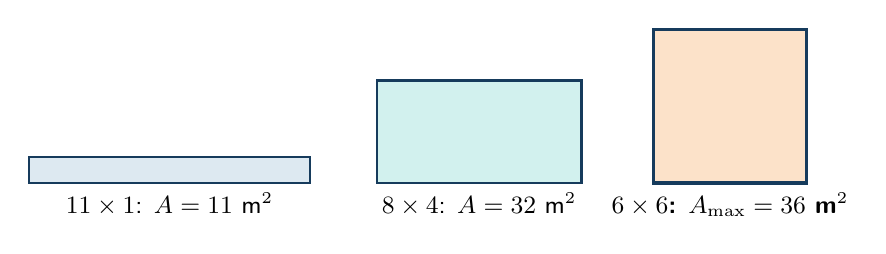
\begin{tikzpicture}[scale=0.65,font=\small]
  \draw[fill=iiiepeBlue!15,draw=iiiepeNavy,thick] (0,0) rectangle (5.5,0.5);
  \node[below] at (2.75,0) {$11\times 1$: $A=11\text{ m}^2$};
  \draw[fill=iiiepeAqua!20,draw=iiiepeNavy,thick] (6.8,0) rectangle (10.8,2.0);
  \node[below] at (8.8,0) {$8\times 4$: $A=32\text{ m}^2$};
  \draw[fill=iiiepeOrange!25,draw=iiiepeNavy,very thick] (12.2,0) rectangle (15.2,3.0);
  \node[below] at (13.7,0) {\textbf{$6\times 6$: $A_{\max}=36\text{ m}^2$}};
\end{tikzpicture}
\end{center}

\textbf{Pausa reflexiva 1 (diapositiva 8):} Si este reto se aplica con estudiantes, emergen cuatro dificultades típicas: (1) asumir que figuras con el mismo perímetro tienen la misma área; (2) excluir el cuadrado $6\times 6$ por creer que ``no es rectángulo''; (3) sumar solamente dos lados ($l+a=24$) olvidando que la cerca rodea los cuatro lados; y (4) contar unidades de contorno confundiendo segmentos con cuadros de esquina. Para ayudarles sin dar la respuesta, el docente debe preguntar: \textit{``Si usamos la cerca solo como una cinta de $24\text{ m}$, ¿cuánto suman un largo y un ancho juntos?'', ``¿Qué ocurre con el espacio interior cuando acercamos el largo y el ancho a un mismo valor?'', ``¿Un cuadrado cumple la definición de rectángulo?''}.

\subsection{Reto 2: El arquitecto bajo presión (Diapositivas 9--10)}
\textbf{Planteamiento:} La escuela desea un jardín rectangular de $A = 48\text{ m}^2$ disponiendo de $P = 28\text{ m}$ de cerca. El director asegura que el material alcanza y exige un diseño que lo demuestre.

\textbf{Resolución y comprobación:} Se busca un par $(l, a)$ que satisfaga simultáneamente $l\cdot a = 48$ y $2(l + a) = 28 \iff l + a = 14$. Estas magnitudes corresponden a las raíces de la ecuación cuadrática:
\[
t^2 - 14t + 48 = 0 \implies (t - 8)(t - 6) = 0 \implies l = 8\text{ m},\quad a = 6\text{ m}.
\]
Comprobando: $A = 8\text{ m} \times 6\text{ m} = 48\text{ m}^2$ y $P = 2(8 + 6) = 28\text{ m}$. Al analizar todas las factorizaciones enteras de $48$: $(48,1)\to P=98\text{ m}$, $(24,2)\to P=52\text{ m}$, $(16,3)\to P=38\text{ m}$, $(12,4)\to P=32\text{ m}$, y $(8,6)\to P=28\text{ m}$, se concluye que \textbf{sí es posible construir el jardín}, y que $8\text{ m} \times 6\text{ m}$ es precisamente la configuración entera de perímetro mínimo ($28\text{ m}$). Incluso en los reales, el límite inferior absoluto sería un cuadrado de lado $\sqrt{48} \approx 6.928\text{ m}$ cuyo perímetro es $4\sqrt{48} \approx 27.71\text{ m} < 28\text{ m}$.

\begin{center}
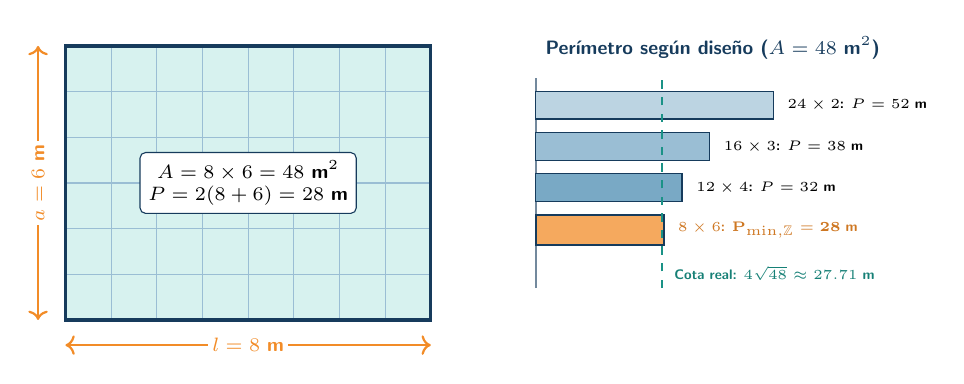
\begin{tikzpicture}[scale=0.58,font=\scriptsize]
  % Rectangulo optimo 8x6 con cuadricula de 48 m^2
  \fill[iiiepeAqua!18] (0,0) rectangle (8,6);
  \draw[step=1,iiiepeBlue!45,thin] (0,0) grid (8,6);
  \draw[very thick,iiiepeNavy] (0,0) rectangle (8,6);
  \draw[<->,thick,iiiepeOrange] (0,-0.55) -- (8,-0.55) node[midway,fill=white,inner sep=1.5pt,font=\scriptsize\bfseries] {$l = 8\text{ m}$};
  \draw[<->,thick,iiiepeOrange] (-0.6,0) -- (-0.6,6) node[midway,fill=white,inner sep=1.5pt,rotate=90,font=\scriptsize\bfseries] {$a = 6\text{ m}$};
  \node[fill=white,draw=iiiepeNavy,rounded corners=2pt,inner sep=3pt,align=center,font=\scriptsize\bfseries] at (4,3) {$A = 8 \times 6 = 48\text{ m}^2$\\$P = 2(8+6) = 28\text{ m}$};

  % Comparativa lateral de factorizaciones de 48 m^2
  \begin{scope}[xshift=10.3cm,yshift=0.3cm]
    \node[above right,font=\scriptsize\bfseries,iiiepeNavy] at (0,5.2) {Perímetro según diseño ($A=48\text{ m}^2$)};
    \draw[iiiepeNavy!60,thick] (0,0.4) -- (0,5.0);
    % Barras horizontales proporcionales (x1 unit = 10 m)
    \fill[iiiepeBlue!30,draw=iiiepeNavy] (0,4.1) rectangle (5.2,4.7);
    \node[right,font=\tiny\bfseries] at (5.3,4.4) {$24\times 2$: $P=52\text{ m}$};
    \fill[iiiepeBlue!45,draw=iiiepeNavy] (0,3.2) rectangle (3.8,3.8);
    \node[right,font=\tiny\bfseries] at (3.9,3.5) {$16\times 3$: $P=38\text{ m}$};
    \fill[iiiepeBlue!60,draw=iiiepeNavy] (0,2.3) rectangle (3.2,2.9);
    \node[right,font=\tiny\bfseries] at (3.3,2.6) {$12\times 4$: $P=32\text{ m}$};
    \fill[iiiepeOrange!75,draw=iiiepeNavy,thick] (0,1.35) rectangle (2.8,2.0);
    \node[right,font=\tiny\bfseries,iiiepeOrange!85!black] at (2.9,1.67) {$8\times 6$: $\mathbf{P_{\min,\mathbb{Z}}=28\text{ m}}$};
    \draw[dashed,iiiepeAqua!80!black,thick] (2.77,0.4) -- (2.77,5.0);
    \node[font=\tiny\bfseries,iiiepeAqua!70!black,right] at (2.82,0.72) {Cota real: $4\sqrt{48}\approx 27.71\text{ m}$};
  \end{scope}
\end{tikzpicture}
\end{center}

\textbf{Pausa reflexiva 2 (diapositiva 10):} Para formar estudiantes capaces de cuestionar y comprobar afirmaciones matemáticas emitidas por una figura de autoridad, la clase debe institucionalizar la \textbf{validación empírica y deductiva como criterio único de verdad}. Esto implica pedir siempre las dos verificaciones simultáneas (``muéstrame en el dibujo o la tabla dónde está la suma de los lados y dónde el conteo de metros cuadrados''), proponer tanto afirmaciones verdaderas como falsas provenientes de personajes ficticios (como el director) para que el alumno ejerza el control de calidad mediante contraejemplos, y legitimar el desacuerdo argumentado.

\subsection{Reto 3: El jardín imposible (Diapositivas 11--13)}
\textbf{Planteamiento:} Se construirá un jardín rectangular adosado a una pared existente (cercando únicamente tres lados con $24\text{ m}$ de malla, esto es, $2a + l = 24\text{ m}$, con $a$ perpendicular a la pared y $l$ paralelo a ella). Se exige que las dimensiones sean \textbf{números enteros de metros}, se utilice toda la cerca y se obtenga un área $A \ge 70\text{ m}^2$.

\textbf{Exploración exhaustiva en $\mathbb{Z}^+$:} Sustituyendo $l = 24 - 2a$ para $a \in \{1,\dots,11\}$:

{\small\setstretch{1.1}\renewcommand{\arraystretch}{1.2}
\begin{longtable}{|>{\centering\arraybackslash}p{0.15\linewidth}|>{\centering\arraybackslash}p{0.20\linewidth}|>{\centering\arraybackslash}p{0.22\linewidth}|>{\centering\arraybackslash}p{0.18\linewidth}|>{\raggedright\arraybackslash}p{0.22\linewidth}|}\hline
\rowcolor{iiiepePale} \textbf{Ancho $a$ (m)} & \textbf{Largo $l=24-2a$} & \textbf{Cerca $2a+l$} & \textbf{Área $A=a\cdot l$} & \textbf{Cumple $A\ge 70\text{ m}^2$} \\\hline
\endfirsthead\hline
\rowcolor{iiiepePale} \textbf{Ancho $a$ (m)} & \textbf{Largo $l=24-2a$} & \textbf{Cerca $2a+l$} & \textbf{Área $A=a\cdot l$} & \textbf{Cumple $A\ge 70\text{ m}^2$} \\\hline
\endhead
$3$ & $18$ & $24\text{ m}$ & $54\text{ m}^2$ & No ($54 < 70$) \\\hline
$4$ & $16$ & $24\text{ m}$ & $64\text{ m}^2$ & No ($64 < 70$) \\\hline
$\mathbf{5}$ & $\mathbf{14}$ & $24\text{ m}$ & $\mathbf{70\text{ m}^2}$ & \textbf{Sí (igual a $70$)} \\\hline
$\mathbf{6}$ & $\mathbf{12}$ & $24\text{ m}$ & $\mathbf{72\text{ m}^2}$ & \textbf{Sí (Área máxima)} \\\hline
$\mathbf{7}$ & $\mathbf{10}$ & $24\text{ m}$ & $\mathbf{70\text{ m}^2}$ & \textbf{Sí (igual a $70$)} \\\hline
$8$ & $8$ & $24\text{ m}$ & $64\text{ m}^2$ & No (cuadrado, pero no óptimo) \\\hline
$9$ & $6$ & $24\text{ m}$ & $54\text{ m}^2$ & No \\\hline
\end{longtable}}

\textbf{Demostración algebraica:} $A(a) = a(24 - 2a) = 24a - 2a^2 = 72 - 2(a - 6)^2 \le 72\text{ m}^2$. Por lo tanto, el llamado ``jardín imposible'' \textbf{sí es posible} en tres configuraciones enteras: $(5\text{ m}\times 14\text{ m})$, $(6\text{ m}\times 12\text{ m})$ y $(7\text{ m}\times 10\text{ m})$. La solución óptima ($6\text{ m}\times 12\text{ m}$, $A_{\max}=72\text{ m}^2$) ya no es un cuadrado sino un rectángulo de razón $2:1$, pues la pared aporta sin costo el cuarto lado y la simetría óptima iguala el gasto de malla en ambas direcciones ($2a = l = 12\text{ m}$).

\begin{figure}[htbp]
\centering
\begin{minipage}[c]{0.47\linewidth}
  \centering
  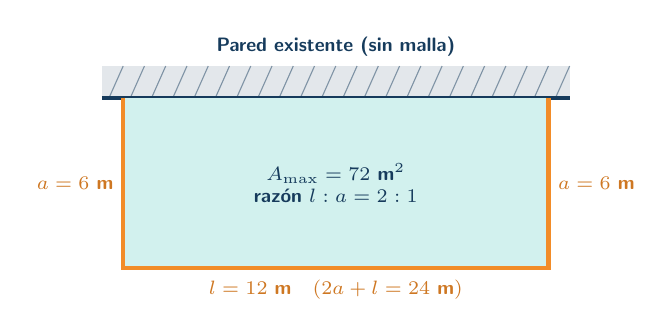
\begin{tikzpicture}[scale=0.45,font=\scriptsize]
    % Muro escolar achurado en la parte superior
    \fill[iiiepeNavy!12] (-0.6,5.2) rectangle (12.6,6.1);
    \foreach \x in {-0.4,0.2,...,12.2}
      \draw[iiiepeNavy!55,thin] (\x,5.2) -- (\x+0.4,6.1);
    \draw[ultra thick,iiiepeNavy] (-0.6,5.2) -- (12.6,5.2);
    \node[above,font=\scriptsize\bfseries,iiiepeNavy] at (6,6.1) {Pared existente (sin malla)};

    % Jardin optimo adosado 12 m x 6 m (y=1.2..5.2 -> escala vertical 4/6 para compacidad, etiquetado exacto)
    \fill[iiiepeAqua!20] (0,0.4) rectangle (12,5.2);
    \draw[ultra thick,iiiepeOrange] (0,5.2) -- (0,0.4) -- (12,0.4) -- (12,5.2);
    \node[left,font=\scriptsize\bfseries,iiiepeOrange!85!black] at (0,2.8) {$a=6\text{ m}$};
    \node[right,font=\scriptsize\bfseries,iiiepeOrange!85!black] at (12,2.8) {$a=6\text{ m}$};
    \node[below,font=\scriptsize\bfseries,iiiepeOrange!85!black] at (6,0.35) {$l = 12\text{ m}\quad(2a+l=24\text{ m})$};
    \node[align=center,font=\scriptsize\bfseries,iiiepeNavy] at (6,2.8) {$A_{\max} = 72\text{ m}^2$\\razón $l:a = 2:1$};
  \end{tikzpicture}
\end{minipage}\hfill
\begin{minipage}[c]{0.50\linewidth}
  \centering
  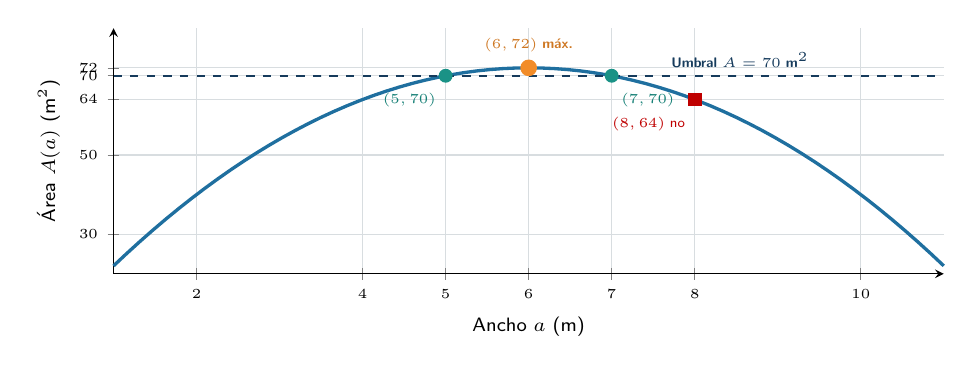
\begin{tikzpicture}
    \begin{axis}[
      width=\linewidth, height=4.7cm,
      xlabel={\scriptsize Ancho $a$ (m)},
      ylabel={\scriptsize Área $A(a)$ ($\text{m}^2$)},
      xmin=1, xmax=11, ymin=20, ymax=82,
      xtick={2,4,5,6,7,8,10},
      ytick={30,50,64,70,72},
      tick label style={font=\tiny},
      grid=both, grid style={iiiepePale!80!gray,thin},
      axis lines=left,
      clip=false
    ]
      \addplot[domain=1:11,samples=65,iiiepeBlue,very thick] {24*x - 2*x^2};
      \addplot[domain=1:11,dashed,iiiepeNavy,thick] {70};
      \node[right,font=\tiny\bfseries,iiiepeNavy] at (axis cs:7.6,74) {Umbral $A=70\text{ m}^2$};
      \addplot[only marks,mark=*,mark size=2.3pt,iiiepeAqua!80!black] coordinates {(5,70) (7,70)};
      \addplot[only marks,mark=*,mark size=2.8pt,iiiepeOrange] coordinates {(6,72)};
      \addplot[only marks,mark=square*,mark size=2.3pt,red!75!black] coordinates {(8,64)};
      \node[above,font=\tiny\bfseries,iiiepeOrange!85!black] at (axis cs:6,73.5) {$(6,72)$ máx.};
      \node[below left,font=\tiny,iiiepeAqua!70!black] at (axis cs:5,68) {$(5,70)$};
      \node[below right,font=\tiny,iiiepeAqua!70!black] at (axis cs:7,68) {$(7,70)$};
      \node[below left,font=\tiny,red!75!black] at (axis cs:8,62) {$(8,64)$ no};
    \end{axis}
  \end{tikzpicture}
\end{minipage}
\caption{Reto 3: Diseño óptimo adosado ($6\text{ m}\times 12\text{ m}$) y curva cuadrática $A(a)=24a-2a^2$ frente al umbral $A\ge 70\text{ m}^2$.}
\end{figure}

\textbf{Pausa reflexiva 3 (diapositiva 13):} Existe una diferencia cualitativa fundamental entre \textbf{aumentar la dificultad de los cálculos} (por ejemplo, emplear decimales como $24.75\text{ m}$ o números grandes sin cambiar la estructura del problema) y \textbf{aumentar la complejidad del razonamiento}. El Reto 3 eleva la complejidad del razonamiento porque altera una restricción estructural (suprimir un lado cercado), lo cual invalida la heurística memorizada del Reto 1 (``el óptimo siempre es un cuadrado'', que aquí da $8\times 8 = 64\text{ m}^2 < 70\text{ m}^2$) y obliga al estudiante a modelar la nueva relación $2a + l = 24$ y justificar existencia y maximalidad.

\section{Propuesta didáctica colaborativa en Canva (Equipo 4)}
En el tablero colaborativo de Canva (\textit{s8 MAEM T.S. Propuestas}), la diapositiva 1 (\textit{Organización}) ubica a \textbf{Jonathan} como integrante 3 del \textbf{Equipo 4} junto con Alejandro Herrera y Christopher de Luna. En la diapositiva 5 (\textit{Equipo 4}), el equipo articuló una propuesta didáctica contextualizada y verificó la solución del Reto 2 ($8\text{ m}\times 6\text{ m}=48\text{ m}^2$).

\begin{figure}[htbp]
\centering
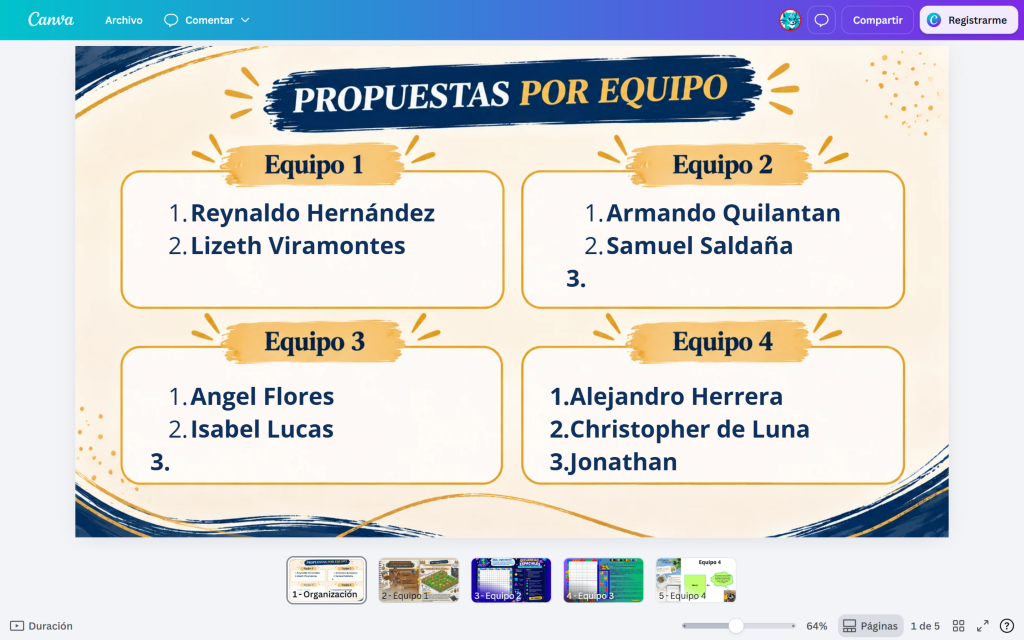
\includegraphics[width=0.86\linewidth]{img/canva/organizacion_equipos.png}
\caption{Evidencia del tablero colaborativo Canva (\textit{1 - Organización}): asignación de Jonathan al Equipo 4.}
\end{figure}

\begin{figure}[htbp]
\centering
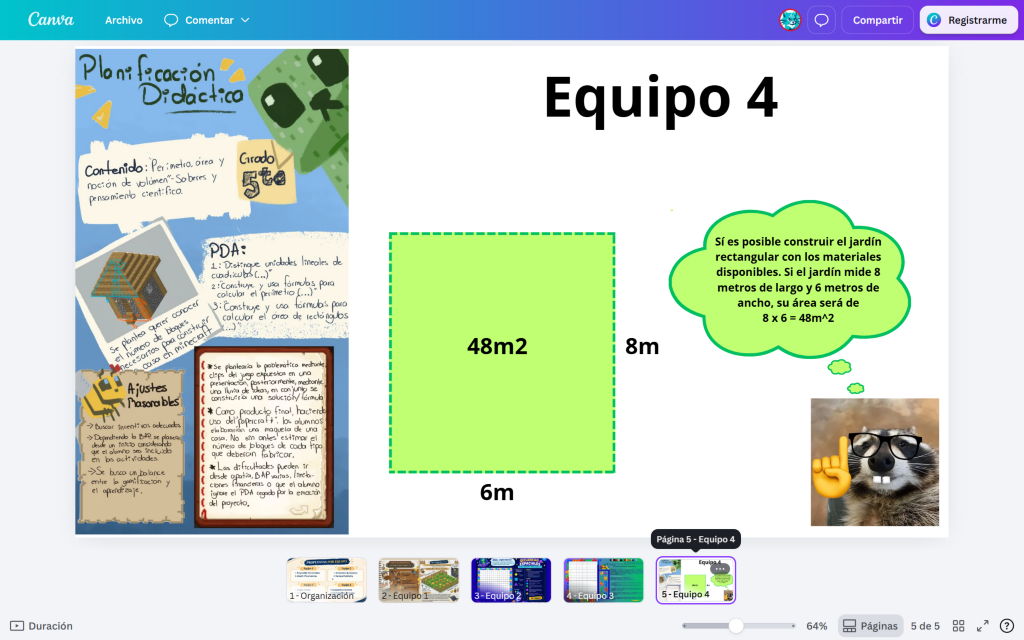
\includegraphics[width=0.86\linewidth]{img/canva/equipo_04_propuesta.png}
\caption{Evidencia del tablero colaborativo Canva (\textit{5 - Equipo 4}): Planificación didáctica de 5.º grado (Minecraft/Papercraft) y comprobación del jardín $8\,\text{m}\times 6\,\text{m}=48\,\text{m}^2$.}
\end{figure}

\subsection{Síntesis estructural de la propuesta del Equipo 4 (criterios de la diapositiva 15)}
\begin{enumerate}
  \item \textbf{Grado escolar y ubicación curricular:} 5.º grado de educación primaria, campo formativo \textit{Saberes y Pensamiento Científico}. Contenidos y Procesos de Desarrollo de Aprendizaje (PDA): (1) distingue unidades lineales de cuadráticas; (2) construye y usa fórmulas para calcular el perímetro; y (3) construye y usa fórmulas para calcular el área de rectángulos.
  \item \textbf{Situación o reto matemático:} A partir de clips del videojuego \textit{Minecraft}, el alumnado enfrenta el desafío de estimar y justificar cuántos bloques cuadrados y lineales necesita para construir la base, barda perimetral y muros de una casa optimizando el terreno disponible (conectado con el problema de cercado y área de $48\text{ m}^2$ con $28\text{ m}$ de perímetro).
  \item \textbf{Estrategia didáctica y materiales:} Lluvia de ideas guiada a partir de secuencias del juego, trabajo colaborativo por retos, hojas cuadriculadas y construcción física final en \textit{papercraft} (maqueta a escala donde primero estiman y justifican la cantidad de bloques de cada tipo antes de recortar y armar).
  \item \textbf{Intervención docente y ajustes razonables:} Anticipación de dificultades (apatía, Barreras para el Aprendizaje y la Participación [BAP], limitaciones de material o distracción lúdica perdiendo de vista el PDA). El docente media mediante preguntas orientadoras sin entregar fórmulas de antemano (\textit{``¿Qué unidades cuentan el contorno y cuáles cubren el piso?'', ``¿Dos casas con la misma barda requieren los mismos bloques de piso?''}) y equilibra gamificación con rigor matemático.
  \item \textbf{Aprendizaje esperado:} Comprensión conceptual diferenciada entre longitud lineal (perímetro) y superficie (área), deducción significativa de las fórmulas del rectángulo y argumentación de sus estimaciones.
\end{enumerate}

\section{Alineación con la Rúbrica de Evaluación (Actividad 1)}
{\small\setstretch{1.08}\renewcommand{\arraystretch}{1.18}
\begin{longtable}{|>{\raggedright\arraybackslash}p{0.25\linewidth}|>{\raggedright\arraybackslash}p{0.71\linewidth}|}\hline
\rowcolor{iiiepePale} \textbf{Criterio (Excelente = 10)} & \textbf{Evidencia integrada en este entregable} \\\hline
\endfirsthead\hline
\rowcolor{iiiepePale} \textbf{Criterio (Excelente = 10)} & \textbf{Evidencia integrada en este entregable} \\\hline
\endhead
1. Participación en los retos matemáticos & Se resuelven y demuestran los retos 1, 2 y 3 con tablas exhaustivas, factorización, completación de cuadrados y diagramas vectoriales. \\\hline
2. Reflexión pedagógica & Se responden las tres pausas reflexivas anticipando obstáculos cognitivos y diferenciando cálculo de complejidad inferencial. \\\hline
3. Grado escolar de la propuesta & 5.º grado de primaria (Saberes y Pensamiento Científico) con tres PDA explícitos. \\\hline
4. Situación o reto matemático & Reto contextualizado en \textit{Minecraft} y \textit{papercraft} más verificación del jardín $8\text{ m}\times 6\text{ m}$. \\\hline
5. Estrategia didáctica y materiales & Lluvia de ideas, cuadrícula, modelado \textit{papercraft} e inclusión de ajustes razonables para BAP. \\\hline
6. Intervención docente & Preguntas orientadoras que promueven autonomía y balance gamificación--aprendizaje sin dar respuestas directas. \\\hline
7. Aprendizaje esperado & Coherencia entre distinción de unidades lineales/cuadráticas, reto constructivo y evaluación formativa. \\\hline
8. Entrega a tiempo & Paquete documental y evidencia visual de Canva completos y validados. \\\hline
\end{longtable}}

\needspace{5\baselineskip}\section*{Referencias}
{\setstretch{1.15}\setlength{\parskip}{6pt}
\par\hangindent=1.27cm\hangafter=1 Instituto de Investigación, Innovación y Estudios de Posgrado para la Educación del Estado de Nuevo León. (2026). \textit{Sesión 8: ¿Qué sabemos y cómo lo enseñamos? Presentación interactiva, tablero colaborativo Canva y rúbrica de evaluación}. EVA Posgrados IIIEPE.
\par\hangindent=1.27cm\hangafter=1 Secretaría de Educación Pública. (2023). \textit{Plan de Estudio para la educación preescolar, primaria y secundaria. Fase 5 (5.º grado)}. SEP.
\par\hangindent=1.27cm\hangafter=1 Van de Walle, J. A., Karp, K. S., \& Bay-Williams, J. M. (2019). \textit{Elementary and middle school mathematics: Teaching developmentally} (10th ed.). Pearson.
}

\end{document}
